\documentclass[12pt,a4paper]{report}
\usepackage{polski}
\usepackage[utf8]{inputenc}
\usepackage{graphicx}
\usepackage{lmodern}
\usepackage[tmargin=2.50cm,bmargin=2.50cm]{geometry}
\usepackage{array}
\usepackage{hyperref}
\hypersetup{
    colorlinks,
    citecolor=black,
    filecolor=black,
    linkcolor=black,
    urlcolor=black
}
\setlength\extrarowheight{2pt} % table,array 

\usepackage{fancyhdr}
 
\pagestyle{fancy}
\fancyhf{}
\lhead{\footnotesize{Dokumentacja projektowa}}
\rhead{\texttt{SportsApp}}
\cfoot{\thepage}
% \rfoot{\footnotesize{}}

\bibliographystyle{abbrv}

\title{\Large{Dokumentacja projektowa}\huge\\SportsApp\\}
\date{\parbox{\linewidth}{\centering%
  ~\endgraf\bigskip
  ~\endgraf\bigskip
  15.06.2018%\today
  \endgraf\bigskip
  AGH, Informatyka WIEiT\\
  \endgraf\bigskip
  Semestr 6\\
  \endgraf\bigskip
  Rok akademicki 2017/18\\
  \endgraf\bigskip}}
  
\author{
  Łukasz Uchman\\
  \href{mailto:luke.uchman@gmail.com}{\texttt{luke.uchman@gmail.com}}\\
  %\texttt{Title}
  \and  
  Krzysztof Gryta\\
  \href{mailto:luke.uchman@gmail.com}{\texttt{luke.uchman@gmail.com}}
  \and  
  Vladyslav Lopatin\\
  \href{mailto:luke.uchman@gmail.com}{\texttt{luke.uchman@gmail.com}}
  \and  
  Jakub Golec\\
  \href{mailto:luke.uchman@gmail.com}{\texttt{luke.uchman@gmail.com}}
}
\renewcommand\thesection{\arabic{section}} % number sections 1,2,3, ...
\usepackage{float}   % H param - don't reposition tables
\restylefloat{table} %
\restylefloat{figure} %
\newcommand{\specialcell}[2][c]{%
  \begin{tabular}[#1]{@{}l@{}}#2\end{tabular}}% by egreg
  
\setcounter{tocdepth}{4}
\setcounter{secnumdepth}{3}


\newcommand*\rot{\rotatebox{90}} % rotate right


% BEGIN %
% https://tex.stackexchange.com/questions/185865/want-to-add-more-column-on-the-left-side

\usepackage{pgfgantt}
\usepackage{rotating}
\usepackage[graphicx]{realboxes}

\newganttchartelement*{mymilestone}{
mymilestone/.style={
shape=isosceles triangle,
inner sep=0pt,
draw=cyan,
top color=white,
bottom color=cyan!50
},
mymilestone incomplete/.style={
/pgfgantt/mymilestone,
draw=yellow,
bottom color=yellow!50
},
mymilestone label font=\slshape,
mymilestone left shift=0pt,
mymilestone right shift=0pt
}

\newgantttimeslotformat{stardate}{%
\def\decomposestardate##1.##2\relax{%
\def\stardateyear{##1}\def\stardateday{##2}%
}%
\decomposestardate#1\relax%
\pgfcalendardatetojulian{\stardateyear-01-01}{#2}%
\advance#2 by-1\relax%
\advance#2 by\stardateday\relax%
}

\usepackage{listings}
\usepackage{color}

\definecolor{darkblue}{rgb}{0,0,0.8}
\definecolor{darkpurple}{rgb}{0.8,0,0.8}
\lstset{
	language=Python,
	showspaces=false,
	basicstyle=\footnotesize\ttfamily,
	xleftmargin=-0.1\textwidth,
	xrightmargin=-0.1\textwidth,
	numbers=left,
	numberstyle=\tiny,
	numbersep=12pt,
	commentstyle=\color{gray},
    frame=single,
    breaklines=true,
    tabsize=4,
    stepnumber=1, % line numbering step
    showstringspaces=false,
    keywordstyle=\color{darkblue},
    stringstyle=\ttfamily\color{red},
    postbreak=\raisebox{0ex}[0ex][0ex]{\ensuremath{\color{red}\hookrightarrow\space}}
}


% END %

%     Strona tytułowa dokumentu (własny standard Zespołu Projektowego):
%        Nazwa dokumentu: Dokumentacja projektowa: "Temat..."
%        Wykonano w ramach  lab. z …, Uczelnia, , kier., rok studiów, semestr, rok ak., itd.
%        Nazwa kodowa systemu, nr wersji, data
%        Wykonawcy: skład zespołu proj. (z adresami mailowymi, tel. kom.), id, logo, itp;
%    wprowadzenie numeracji stron (bez strony tytułowej);
%    podstawowa czcionka dokumentacji: Times New Roman 12, z odstępem 1,5;
%    umieszczenie spisu treści na drugiej stronie dokumentacji;
%    należy stosować referencje do źródeł (literatury, linków, standardów, itp.); ew. przypisy
%    wszystkie strony, (z wyjątkiem tytułowej), mają być opatrzone stopką i nagłówkiem 
%         w nagłówku strony umieszczenie imion, nazwisk, nr grupy/tematu
%        % w stopce napisu: IO, 2018; 
\begin{document}

\maketitle

\tableofcontents
\newpage
\section{Sformułowanie zadania projektowego}

\subsection{Temat i cel zadania projektowego}

Celem jest stworzenie aplikacji na urządzenia mobilne (Android) ułatwiającej organizację wydarzeń sportowych w najbliższej okolicy. Aplikacja przeznaczona jest dla wszystkich osób szukających ludzi do wspólnego aktywnego spędzania czasu.\\

Jednym z głównych założeń aplikacji jest promowania aktywności fizycznej. W wielu przypadkach osoby, które przykładowo chętnie zagrałyby w siatkówkę lub inny sport drużynowy są ograniczone brakiem odpowiedniej ilości osób do tej aktywności. Aplikacja ułatwi to użytkownikom, a nawet pozwoli nawiązać nowe znajomości.

\subsection{Opis dziedziny problemu}

Aplikacja powinna w przejrzysty sposób udostępniać użytkownikowi możliwość przeglądania dostępnych na mapie świata wydarzeń sportowych, dołączenie do nich, ich organizację i komunikację w ramach grupy zrzeszanej przez konkretne wydarzenie.

\subsection{Opis istniejących rozwiązań, analiza na podstawie źródeł}

\subsubsection{Istniejące rozwiązania}

\begin{enumerate}

\item \texttt{Endomondo}\footnote{\url{https://play.google.com/store/apps/details?id=com.endomondo.android}}
\begin{itemize}
\item Aplikacja również nastawiona na aktywność fizyczną.
\item Nie udostępnia funkcji społecznościowych.
\item Ukierunkowana jest w stronę monitorowania swoich osiągnięć podczas treningu. Nie pełni funkcji sieci społecznościowej.
\item Duża popularność.
\end{itemize}

\item \texttt{WeSport Social Sport App}\footnote{\url{https://play.google.com/store/apps/details?id=com.my.game.wesport}}
\begin{itemize}
\item Aplikacja jest dostępna w Google Play. 
\item Nie zyskała dużej popularności. 
\item Nie jest rozwijana od maja 2017 roku. 
\item Włącza się, lecz nie udostępnia już swoich funkcjonalności - prawdopodobnie wygasł token GoogleMaps API
\item Analizując działanie aplikacji natrafiliśmy na bugi, które nie są spowodowane wygaśnięciem używanych API np. w trakcie wylogowania aplikacja zawiesza się.
\end{itemize}

\end{enumerate}

\subsubsection{Podsumowanie}

Poszukując podobnych aplikacji w internecie oraz \texttt{Google Play}\footnote{\url{https://play.google.com/store?hl=pl}} znaleźliśmy tylko jedną aplikację, która jest bardzo podobna do naszej koncepcji - aplikacja WeSport. Ma ona jednak dużo błędów i aktualnie jest praktycznie niezdatna do użytku zapewne z powodu wygaśnięcia licencji używanych w niej API. Z kolei inne aplikacje typu Endomondo przeznaczone dla podobnej gruby docelowej jak nasza aplikacja są skierowane głównie na mierzenie osiągnięć i wyznaczanie celów niż na zrzeszanie ludzi w celu uprawiania sportu.

% \subsection{Dobór procesu wytwórczego}

% TODO

\subsection{Wstępny harmonogram prac, podział czynności}

Prace planujemy podzielić na dwa zespoły:
\begin{itemize}
\item Zespół zajmujący się frontend'em
\item Zespół zajmujący się backend'em
\end{itemize}

Do końca kwietnia 2018 roku planujemy zapoznać się z problemem, stworzyć wizję oraz wybrać i zapoznać się z używanymi technologiami. Na koniec czerwca planujemy wykonanie pierwszego działającego prototypu aplikacji. Dalsze prace implementacyjne planujemy prowadzić w czasie wakacji aż do października, w którym powstanie finalna wersja środowiska. Następnie planujemy, krótki okres czasu na testowanie  Dokumentacja będzie rozwijana równolegle, w trakcie fazy implementacyjnej i testów.

\newpage
\section{Opis wizji rozwiązania}

\subsection{Wstęp}

W poniższej sekcji przedstawimy naszą wizję rozwiązania. Zaproponujemy architekturę...\\
Projekt planujemy w całości zrealizować w języku Java.

% TODO

\subsection{Model wizji systemu}
% (Poglądowy rysunek: architektura systemu)

\begin{figure}[H]
\centering
\caption{Poglądowy rysunek: architektura systemu.}
\label{im_overview}
\hspace*{0cm}
\scalebox{0.8}{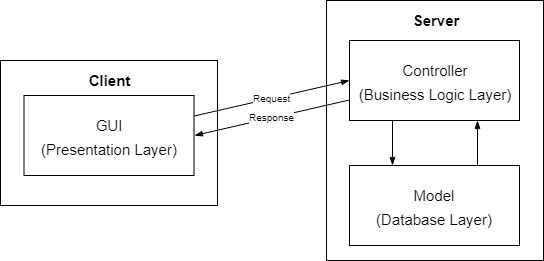
\includegraphics{images/Overview.png}}
\end{figure}

Architekturę systemu planujemy oprzeć na wzorcu architektonicznym MVC, który idealnie wpasowuje się w wymagania naszego projektu.

\subsection{Ocena ryzyka}

\begin{table}[H]
\centering
\hspace{-1cm}
\caption{Ocena ryzyka}
%\label{my-label}
\begin{tabular}{ | p{4cm} | p{2cm} | p{2cm} | p{2cm} | p{4cm} |}
\hline
Ryzyko & Ramy czasowe & Szansa wystąpienia & Wpływ na projekt & Przeciwdziałanie \\ \hline
    Zmiana stosowanej technologii & kwiecień-maj & wysoka & niski & Dokładna analiza wybranych technologii w fazie planowania \\ \hline
	Opóźnienie w stosunku do harmonogramu & cały czas trwania projektu & średnia & średni & Odpowiednie zaplanowanie prac \\ \hline
\end{tabular}
\end{table}

\subsection{Harmonogram prac (diagram Gantta)}

% TODO harmonogram

\hspace{-3.3cm}
\scalebox{0.90}{
\begin{ganttchart}[x unit=1cm,
vgrid,
hgrid,
bar label node/.append style={rotate=0},
group label node/.append style={rotate=0}]{1}{17}
\gantttitle{Marzec}{4}
\gantttitle{Kwiecień}{5}
\gantttitle{Maj}{4}
\gantttitle{Czerwiec}{4}\\
\gantttitlelist{5.03,12.03,19.03,26.03,
				2.04,9.04,16.04,23.04,30.04,
				7.05,14.05,21.05,28.05,
				4.06,11.06,18.06,25.06}{1}\\

\ganttgroup{Część projektowa}{1}{7} \\

\ganttbar{Wstępne planowanie}{1}{3} \\
\ganttbar{Analiza wymagań}{3}{4} \\
\ganttbar{Architektura systemu}{4}{5} \\
\ganttbar{Mockupy GUI}{6}{6} \\
\ganttbar{Prezentacja otwierająca}{5}{6} \\

\ganttgroup{Implementacja}{6}{15} \\

\ganttbar{TODO}{6}{15} \\
\ganttbar{Prezentacja prototypu}{16}{16} \\
\ganttbar{TODO}{15}{15} \\

%\ganttlink{elem1}{elem2}
%\ganttmilestone{Milestone 1}{11}
\end{ganttchart}
%\end{sidewaysfigure}
}

% TODO opis diagramu Gantta

\end{document}
